\chapter{Implementacija i korisničko sučelje}
		
		\section{Korištene tehnologije i alati}
		
			Komunikacija u timu realizirana je korištenjem aplikacija \underline{WhatsApp}\footnote{https://www.whatsapp.com/} i \underline{Discord} \footnote{https://discord.com/}. Za izradu	UML dijagrama korišten je alat \underline{Astah UML} \footnote{https://astah.net/products/astah-uml/}  , a kao sustav za upravljanje izvornim kodom \underline{Git}\footnote{https://git-scm.com/}. Udaljeni repozitorij projekta je dostupan na web platformi \underline{GitLab} \footnote{https://gitlab.com/} .
			Kao razvojno okruženje korišten je \underline{Visual Studio Code}\footnote{https://code.visualstudio.com/}. Prvenstveno se koristi kao uređivač teksta pri razvoju računalnih programa za operacijski sustav Windows, kao i za web-stranice, web-aplikacije, web-usluge i mobilne aplikacije. Aplikacija je napisana koristeći radni okvir \underline{Flask}\footnote{https://flask.palletsprojects.com/en/2.0.x/} i web poslužitelj \underline{Gunicorn}\footnote{https://gunicorn.org/} u jeziku \underline{Python 3.8}. \footnote{https://www.python.org/} za izradu backenda. Za izradu frontenda su se koristili razvojni okvir \underline{React}\footnote{https://reactjs.org/} i jezik \underline{JavaScript}\footnote{https://www.javascript.com/}. React, takoder poznat kao React.js ili ReactJS, je biblioteka u JavaScriptu za izgradnju korisničkih sučelja. React se najčešće koristi kao osnova	u razvoju web ili mobilnih aplikacija. Složene aplikacije u Reactu obično zahtijevaju korištenje dodatnih biblioteka za interakciju s API-jem. Web poslužitelj Gunicorn nadograđuje radni okvir Flask kako bi mogao posluživati više zahtjeva u isto vrijeme. Naša cijela infrastruktura se nalazi u oblaku na privatnom VPS poslužitelju, poslužuje zahtjeve pomoću \underline{NGINX}\footnote{https://nginx.org/en/} web poslužitelja na linux  ubuntu sustavu.
			Mrežna potpora našoj arhitekturi je \underline{CloudFlare} \footnote{https://www.cloudflare.com/} koja nam nudi usluge poput predmemorije (engl. cache) i DDoS zaštite. Bitan dio naše infrastrukture je baza podataka realizirana kroz \underline{PostgreSQL RDBMS}\footnote{https://www.postgresql.org/}.
			
			
			\eject 
		
	
		\section{Ispitivanje programskog rješenja}
		
			 Svi testovi izvršeni su pomoću skripte u Pythonu koristeći Selenium WebDriver i pytest. Ispitivanje se radilo po obrascima uporabe kako bi se provjerila osnovna funkcionalnost sustava, ali i nasumičnim kretanjima po aplikaciji kako bi se pronašle neočekivane greške(”bugovi”) ili nepredviđena ponašanja. Svaki dio sustava je ispitan, no zbog jednostavnosti u dokumentaciji će biti prikazan samo dio ispitivanja.
	
			
			\subsection{Ispitivanje komponenti}
			\textbf{Ispitni slučajevi}: \newline
			Provedeno je ispitivanje jedinca za 6 ispitnih slučajeva. Ti su slučajevi redom:
			\begin{enumerate}
				\item Konekcija na bazu podataka
				\item Provjera postojanja korisnika
				\item Dohvaćanje imena klase natjecanja
				\item Dohvaćanje zadatka
				\item Dohvaćanje imena zadatka
				\item Dohvaćanje virtualnog natjecanja
			\end{enumerate}
			
			\noindent  \textbf{Očekivani rezultati}: 
			\begin{enumerate}
				\item Uspješna spajanje s bazom podataka
				\item Uspješno/Neuspješno postojanje korisnika ovisno o parametrima
				\item Uspješno dohvaćanje imena klase natjecanja
				\item Uspješno dohvaćanje zadatka
				\item Uspješno dohvaćanje punog imena zadatka
				\item Uspješno dohvaćanje virtualnog natjecanja
			\end{enumerate}
			
			\begin{figure}[H]
				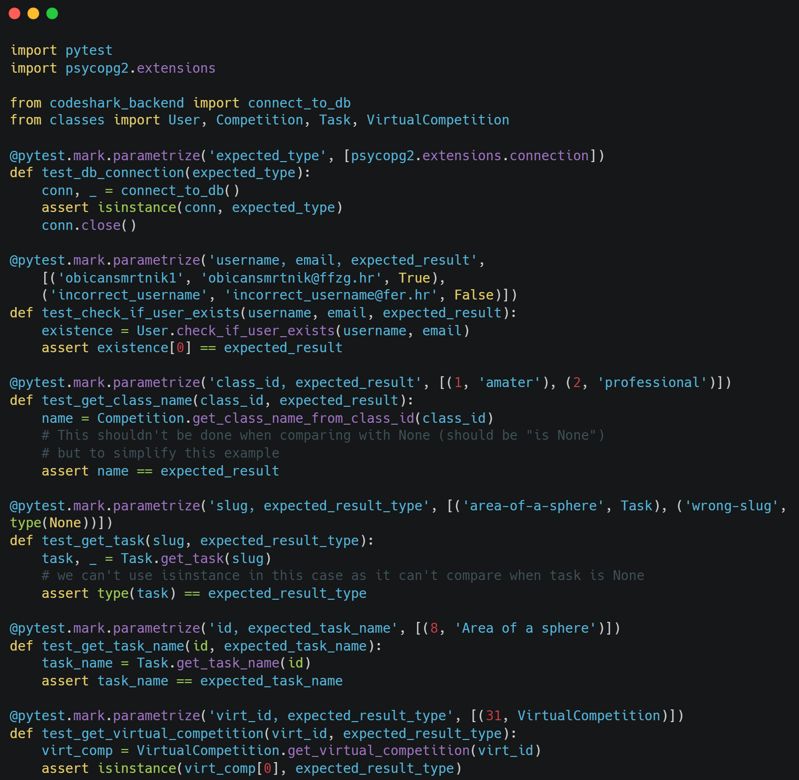
\includegraphics[width=\textwidth]{slike/IspitivanjeKomponenti.png} %veličina u odnosu na širinu linije
				\caption{Ispitivanje komponenti}
				\label{fig:IspitivanjeKomponenti} %label mora biti drugaciji za svaku sliku
			\end{figure}
		
			\begin{figure}[H]
				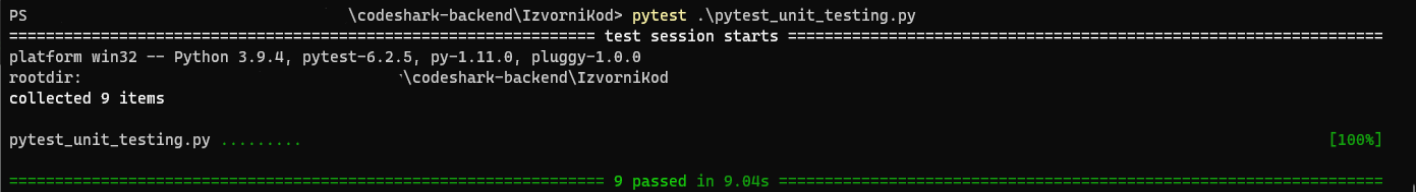
\includegraphics[width=\textwidth]{slike/IspitivanjeKomponentiRez.png} %veličina u odnosu na širinu linije
				\caption{Rezultat ispitivanja komponenti}
				\label{fig:IspitivanjeKomponentiRez} %label mora biti drugaciji za svaku sliku
			\end{figure}
		
			\noindent \textbf{Rezultat}: 
			\newline 
			Svi očekivani rezultati su zadovoljeni.
			
			
			
			\subsection{Ispitivanje sustava}
			\textbf{Ispitni slučajevi}: \newline
			Provedeno je ispitivanje jedinca za 6 ispitnih slučajeva. Ti su slučajevi redom:
			\begin{enumerate}
				\item Dohvaćanje početne stranice
				\item Dohvaćanje popisa korisnika od strane neregistriranog korisnika
				\item Dohvaćanje popisa korisnika od strane registriranog korisnika
				\item Testiranje prijave
				\item Dohvaćanje profilne stranice od strane neregistriranog korisnika
				\item Dohvaćanje profilne stranice od strane registriranog korisnika
			\end{enumerate}
			
			\noindent  \textbf{Očekivani rezultati}: 
			\begin{enumerate}
				\item Stranica je uspješno dohvaćena
				\item Stranica preusmjeruje na stranicu prijave
				\item Stranica je uspješno dohvaćena
				\item Uspješna/Neuspješna prijava ovisno o parametrima
				\item Stranica preusmjeruje na stranicu prijave
				\item Stranica je uspješno dohvaćena
			\end{enumerate}
			
			\begin{figure}[H]
				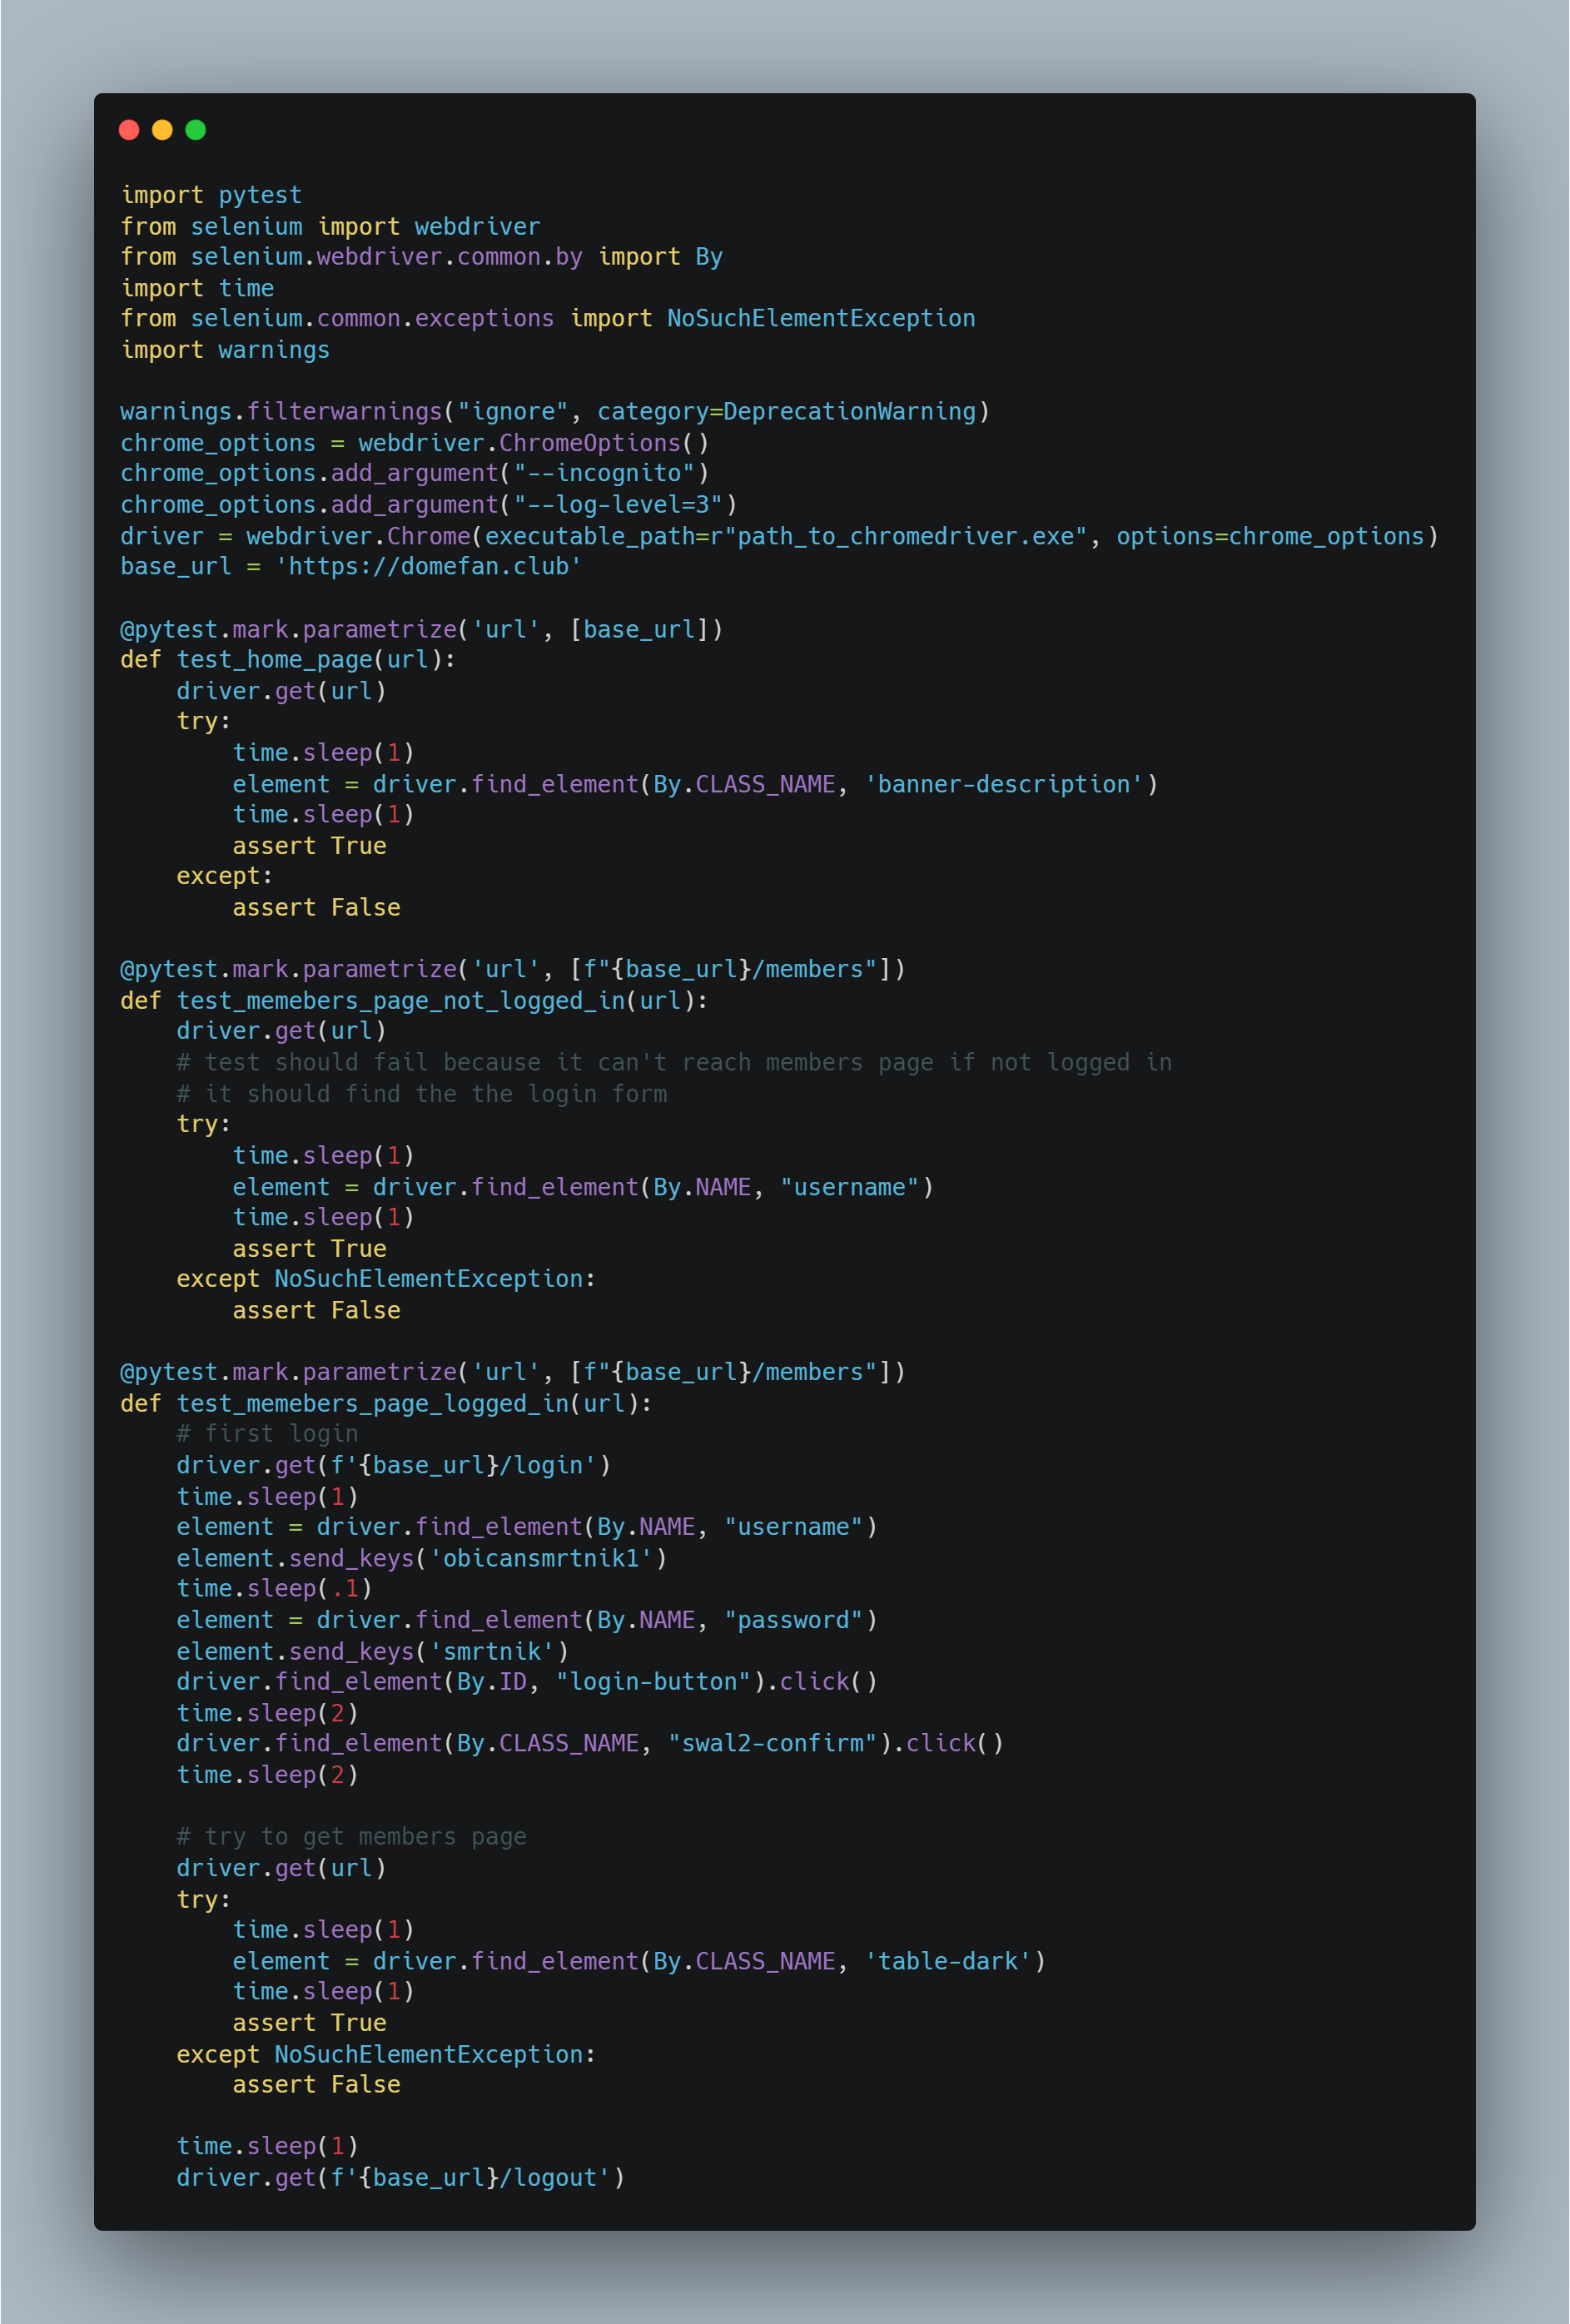
\includegraphics[width=\textwidth]{slike/IspitivanjeSustavaPrviDio.png} %veličina u odnosu na širinu linije
				\caption{Ispitivanje sustava prvi dio}
				\label{fig:IspitivanjeSustavaPrviDio} %label mora biti drugaciji za svaku sliku
			\end{figure}
			\begin{figure}[H]
				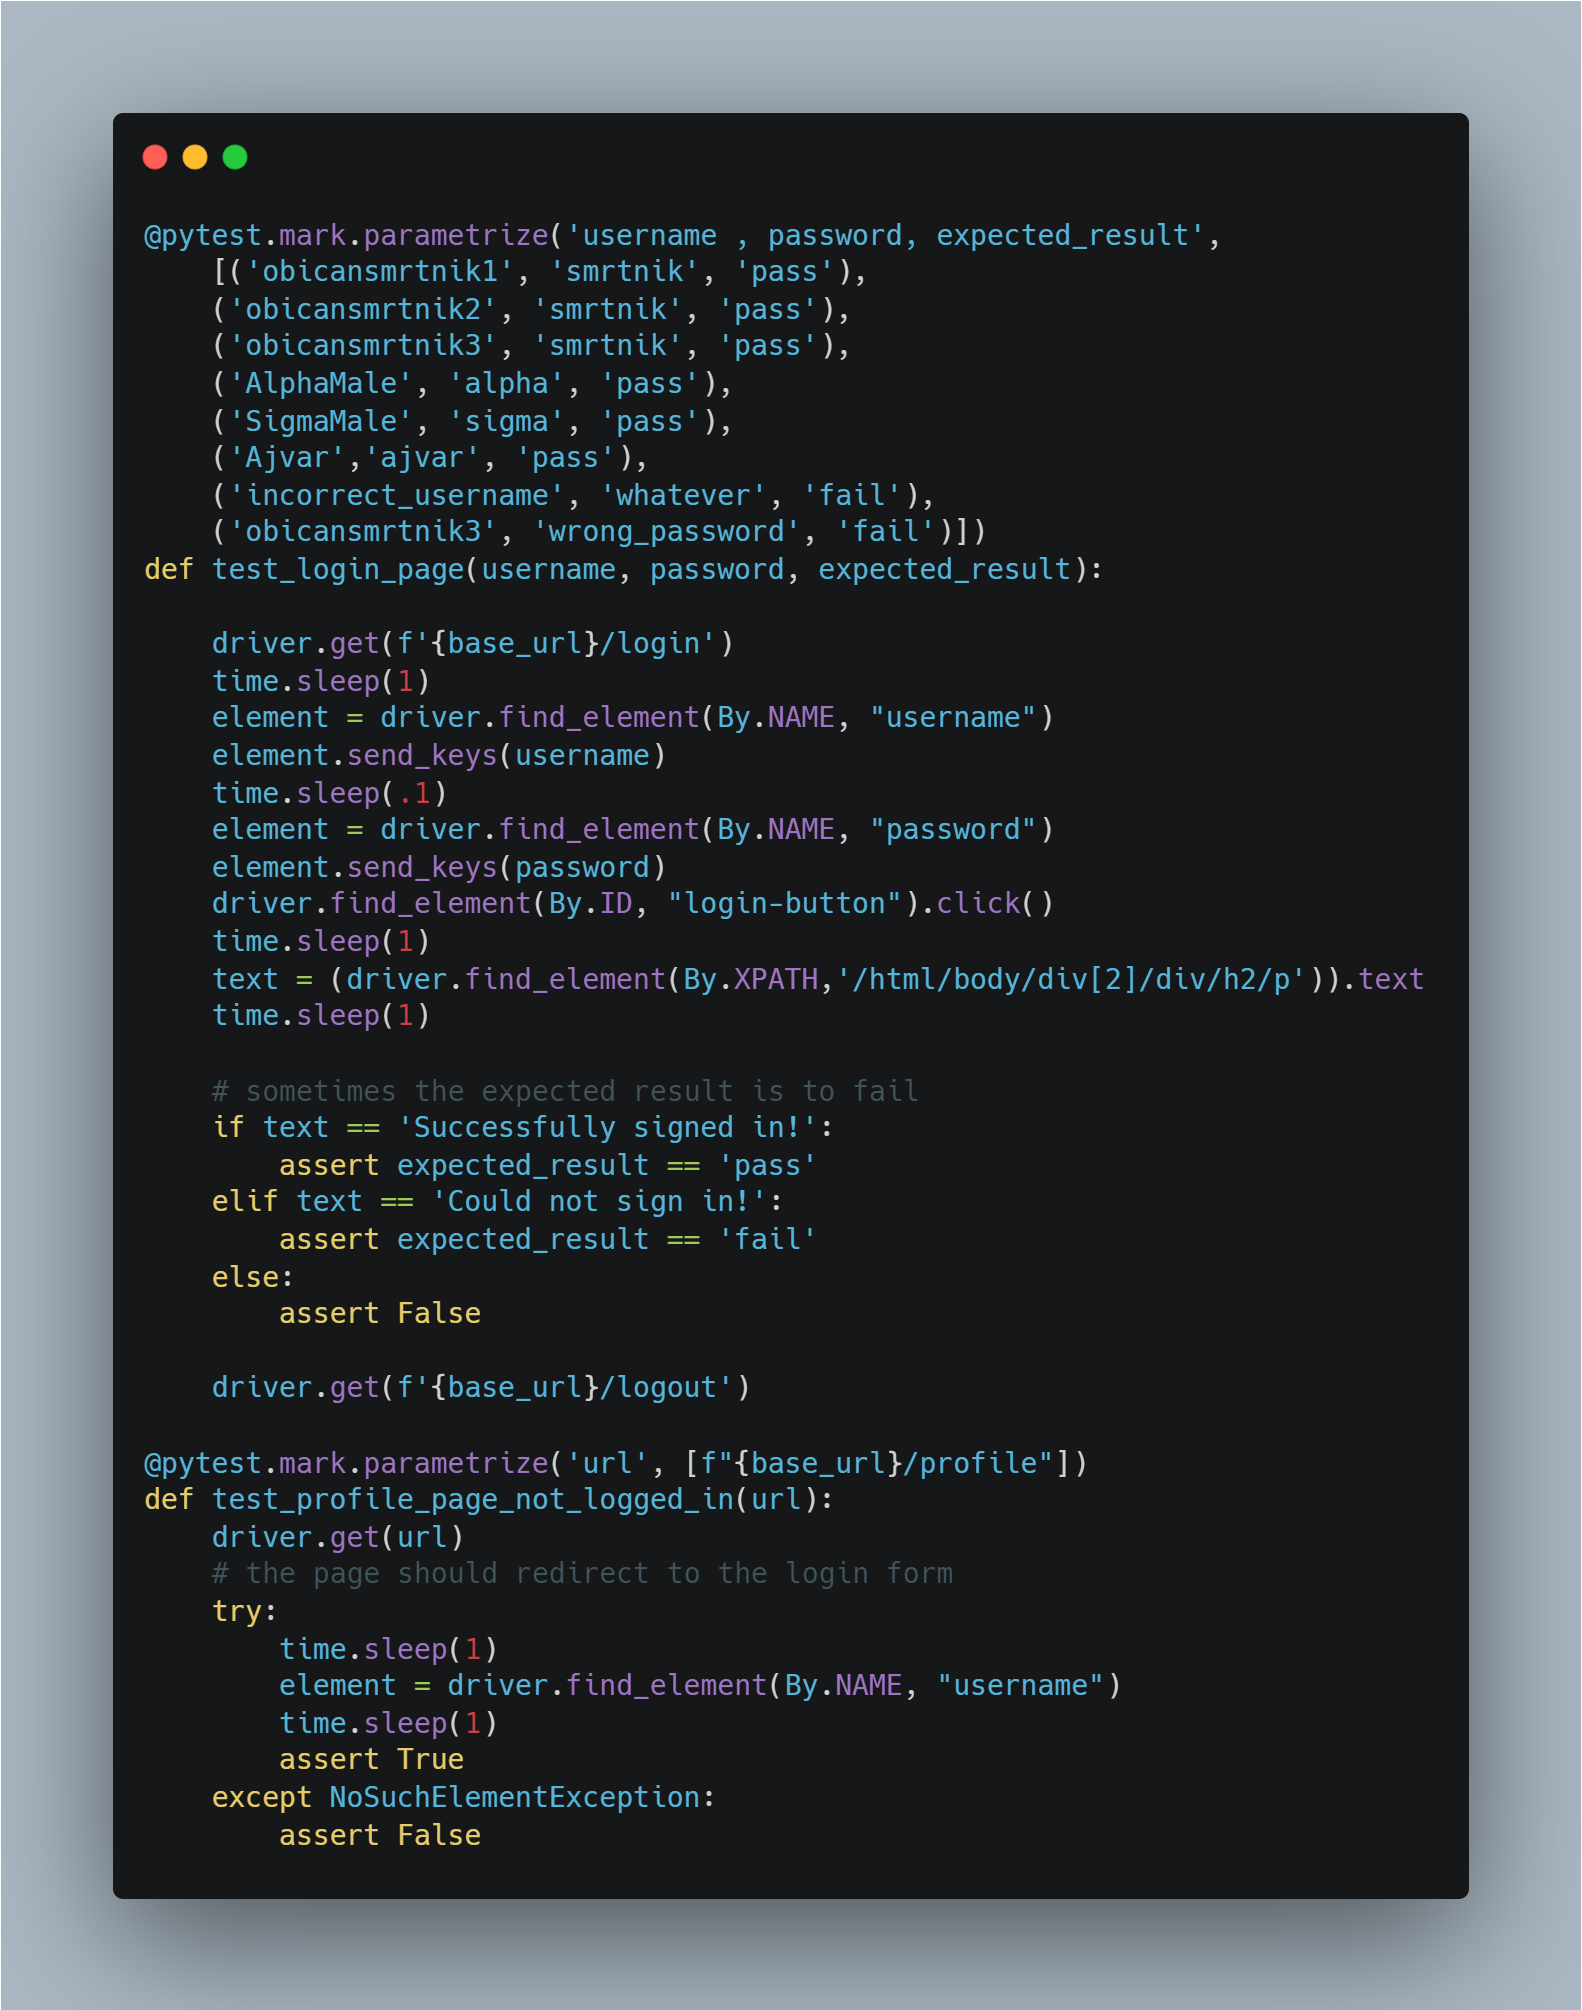
\includegraphics[width=\textwidth]{slike/IspitivanjeSustavaDrugiDio.png} %veličina u odnosu na širinu linije
				\caption{Ispitivanje sustava drugi dio}
				\label{fig:IspitivanjeSustavaDrugiDio} %label mora biti drugaciji za svaku sliku
			\end{figure}
		
			\begin{figure}[H]
				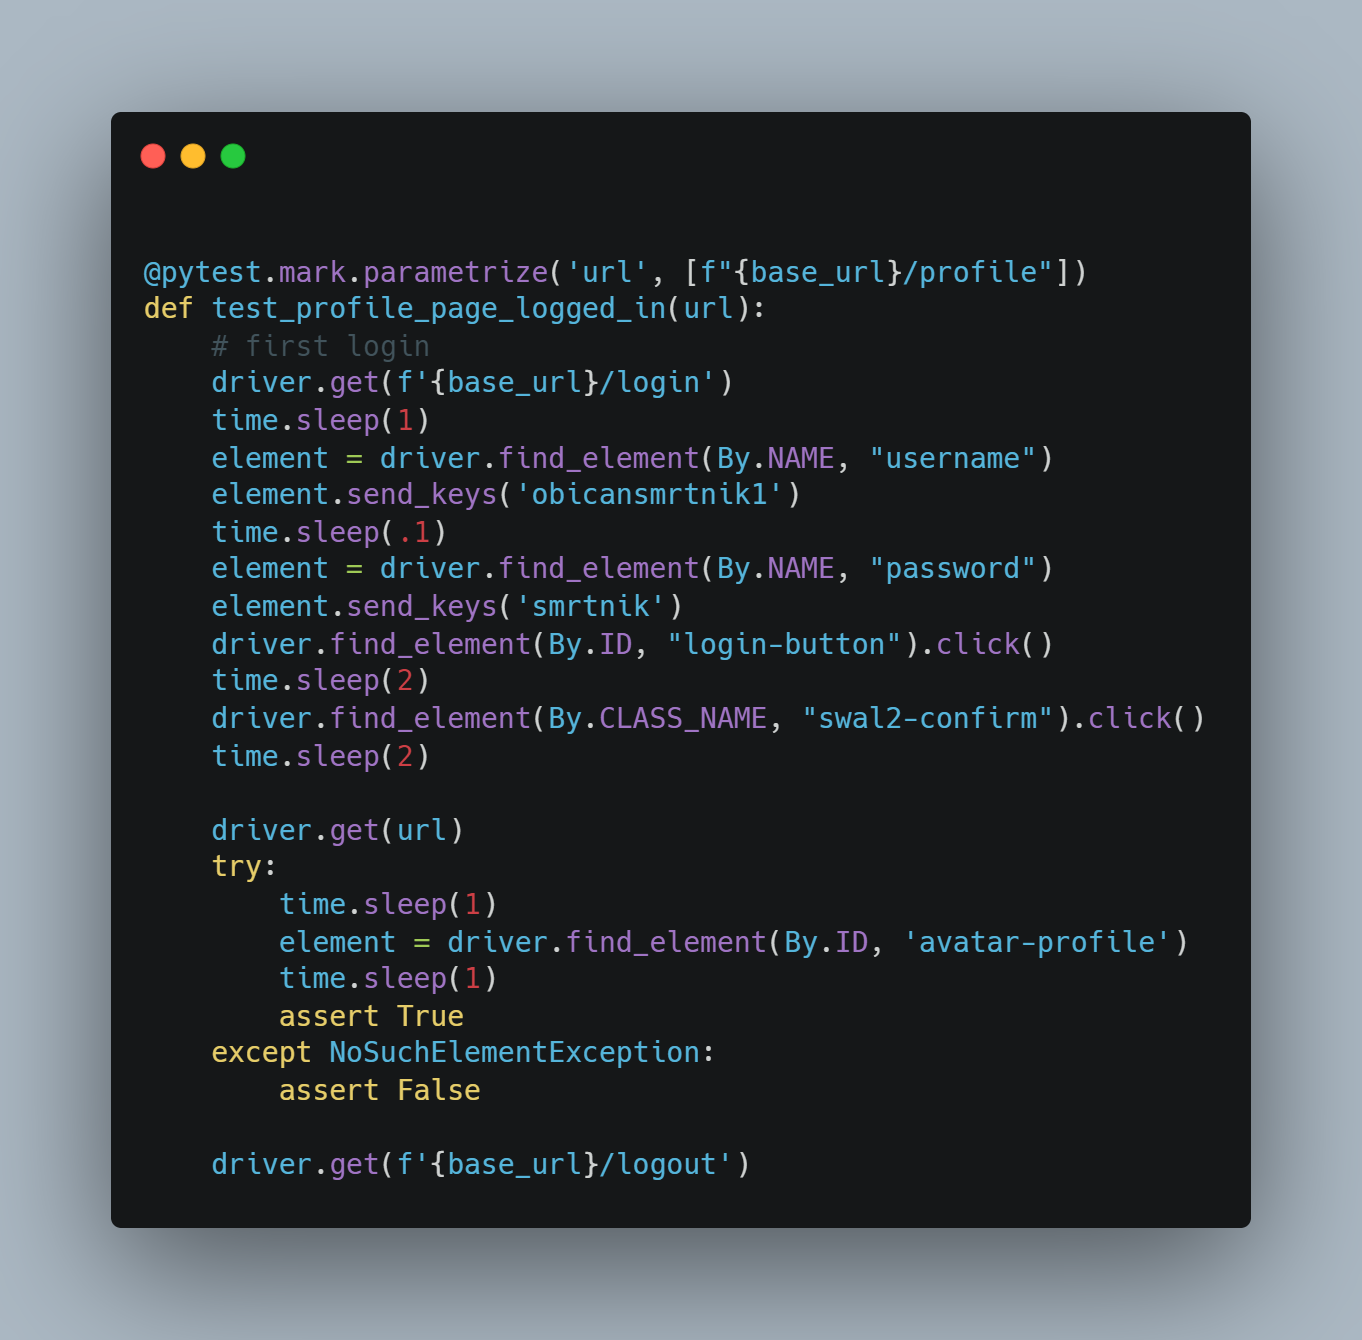
\includegraphics[width=\textwidth]{slike/IspitivanjeSustavaTreciDio.png} %veličina u odnosu na širinu linije
				\caption{Ispitivanje sustava treći dio}
				\label{fig:IspitivanjeSustavaTrećoDio} %label mora biti drugaciji za svaku sliku
			\end{figure}
			
			\begin{figure}[H]
				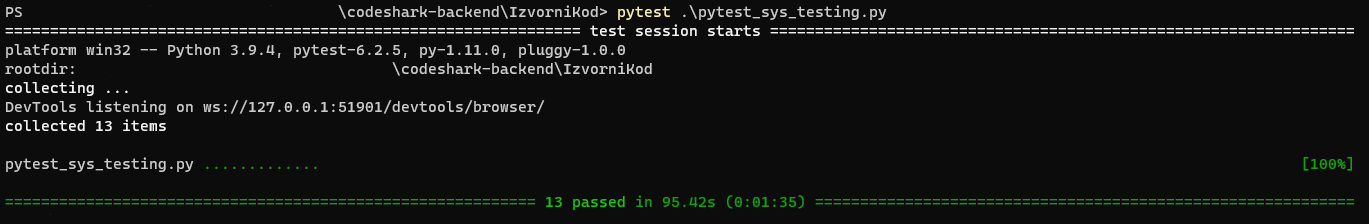
\includegraphics[width=\textwidth]{slike/IspitivanjeSustavaRez.png} %veličina u odnosu na širinu linije
				\caption{Rezultat ispitivanja sustava}
				\label{fig:IspitivanjeSustavaRez} %label mora biti drugaciji za svaku sliku
			\end{figure}
			
			\noindent  \textbf{Rezultat}: \newline
			Svi očekivani rezultati su zadovoljeni.
			 
			 
			
			\eject 
		
		
		\section{Dijagram razmještaja}
			
			Dijagrami razmještaja opisuju topologiju sklopovlja i programsku potporu koja se koristi u implementaciji sustava u njegovom radnom okruženju. Na poslužiteljskom računalu se nalaze web poslužitelj i poslužitelj baze podataka. Klijenti koriste web preglednik kako bi pristupili web aplikaciji. Sustav je baziran na arhitekturi ”klijent – poslužitelj”, a komunikacija između računala korisnika (klijent, zaposlenik, vlasnik, administrator) i poslužitelja odvija se preko HTTPS veze.
			
			
			\begin{figure}[H]
				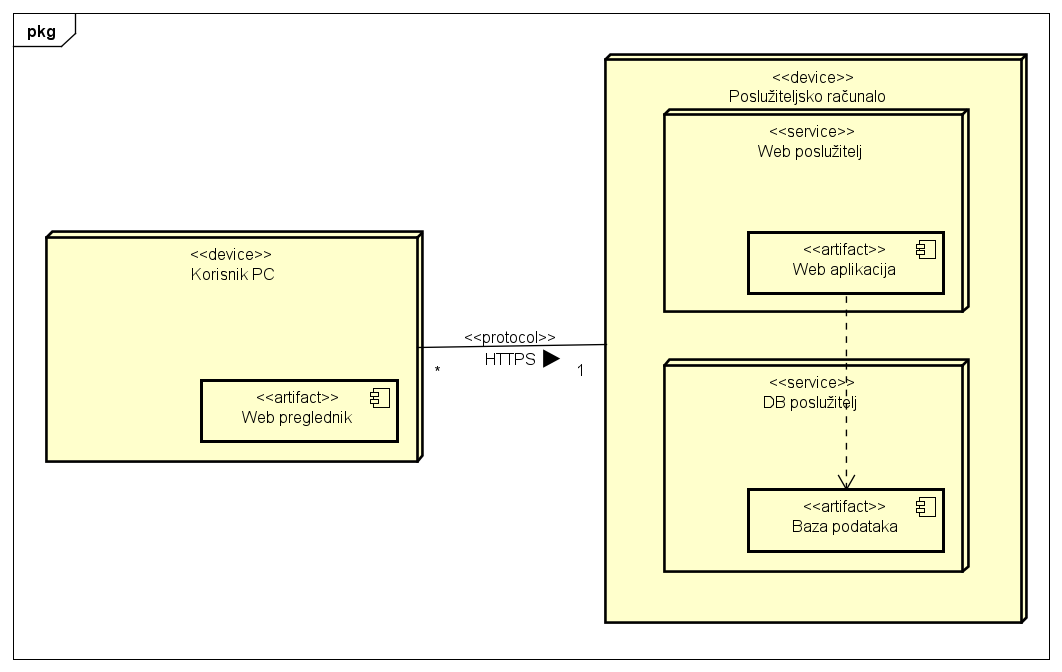
\includegraphics[width=\textwidth]{slike/DijagramRazmjestaja.png} %veličina u odnosu na širinu linije
				\caption{Dijagram Razmještaja}
				\label{fig:DijagramRazmještaja} %label mora biti drugaciji za svaku sliku
			\end{figure}
			
			\eject 
		
		\section{Upute za puštanje u pogon}
		
		
			
			Ove upute su prilagođene očekivanom produkcijskom okruženju softverskih aplikacija. U našem slučaju to znači izvođenje na Linux platformi.
			
			\textbf{Instalacija poslužitelja baze podataka}\\
			
			Potrebno je preuzeti PostgreSQL server za Linux ubuntu platformu.
			Nakon preuzimanja softverske podrške za trenutnu platformu potrebno je postaviti korisnika te bazu podataka na koju taj korisnik ima pristup.\newline
			
			
			\textbf{Konfiguracija DBMS poslužitelja}\\
			
			Nakon uspješne instalacije DBMS poslužitelja potrebno je postaviti host i port. Preporučeno je zatvoriti defaultni Postgres port (5432) na razini sustava kako nitko iz vana ne bi mogao pristupiti bazi.
			Dapače moguće je i otvoriti port Postgres baze u sustavskom vatrozidu tijekom razvoja aplikacije kako bi programeri imali olakšani pristup sustavu.
			Poslužitelj baze podataka radi kao servis kada ga instaliramo u CLI okruženju (što je standardan postupak) te ga ovisno o distribuciji servera možemo ponovno pokrenuti ili zaustaviti pomoću jedne jednostavne naredbe (npr. \textit{service postgres start}).\newline
			
			
			\textbf{Punjenje baze podataka}
			
			Punjenje baze podataka jest doista jednostavno. Uz preuzetu datoteku dump.sql možemo izvršiti jednostavnu naredbu u terminalu \textit{psql -U username dbname < dbexport.pgsql}\newline
			
			
			\textbf{Web poslužitelj NGINX}
			
			U našoj implementaciji koristimo web poslužitelj NGINX kojime obrađujemo dolazne HTTP zahtjeve i usmjerujemo ih ka pravom odredištu. Ovo nije potpuno nužno za pokretanje aplikacije no preporučeno je kako bi se osigurali stilizirani linkovi na samu aplikaciju.
			Kod postavljanja tzv. Server blockova za poslužitelj moramo obratiti pozornost da dolazne zahtjeve preusmjerimo na ispravan port. NGINX Web poslužitelj je vrlo često instaliran već na poslužiteljima baziranima na linux operacijskom sustavu. Alternativno NGINX-u postoji Apache web poslužitelj koji ispunjava istu ulogu.
			
			Unutar direktorija /var/www/ se tipično nalaze datoteke koje web poslužitelj poslužuje na vanjske zahtjeve. Svaka domena na sustavu ima svoju pod-mapu.
			
			Frontend naše aplikacije izgrađen je u React razvojnom okruženju što nam osigurava mogućnost građenja statičkih minimiziranih datoteka koje su spremne za posluživanje. To osigurava dugotrajnost i stabilnost aplikacije. Naredbom "npm run build" možemo izgraditi verziju frontenda spremnu za produkcijsko okruženje.
			Bitna napomena kod ovog koraka pokretanja aplikacije jesu konfiguracijske varijable, ".env.production" te ".env.development". One sadrže bitne informacije poput adrese poslužitelja te poveznica do određenih resursa.
			
			Tijekom lokalnog razvoja moguće je pokrenuti naredbu "npm start" kojom aplikaciju dižemo na lokalnom računalu u svrhu razvoja.\newline
			
			\textbf{Backend sustav}
			
			Backend infrastruktura naše aplikacije bazirana je na Flask i Gunicorn razvojnim okruženjima u jeziku python. Prije pokretanja je bitno prilagoditi konfiguracijske varijable u datoteci "codeshark.cfg". Tamo se nalaze informacije o putanjama na disku za pohranu, podaci za pristup bazi podataka itd. Nakon ispravne konfiguracije te datoteke moguće je pokrenuti backend naredbom "gunicorn --config gunicorn\_config.py".\newline
			
			\begin{figure}[H]
				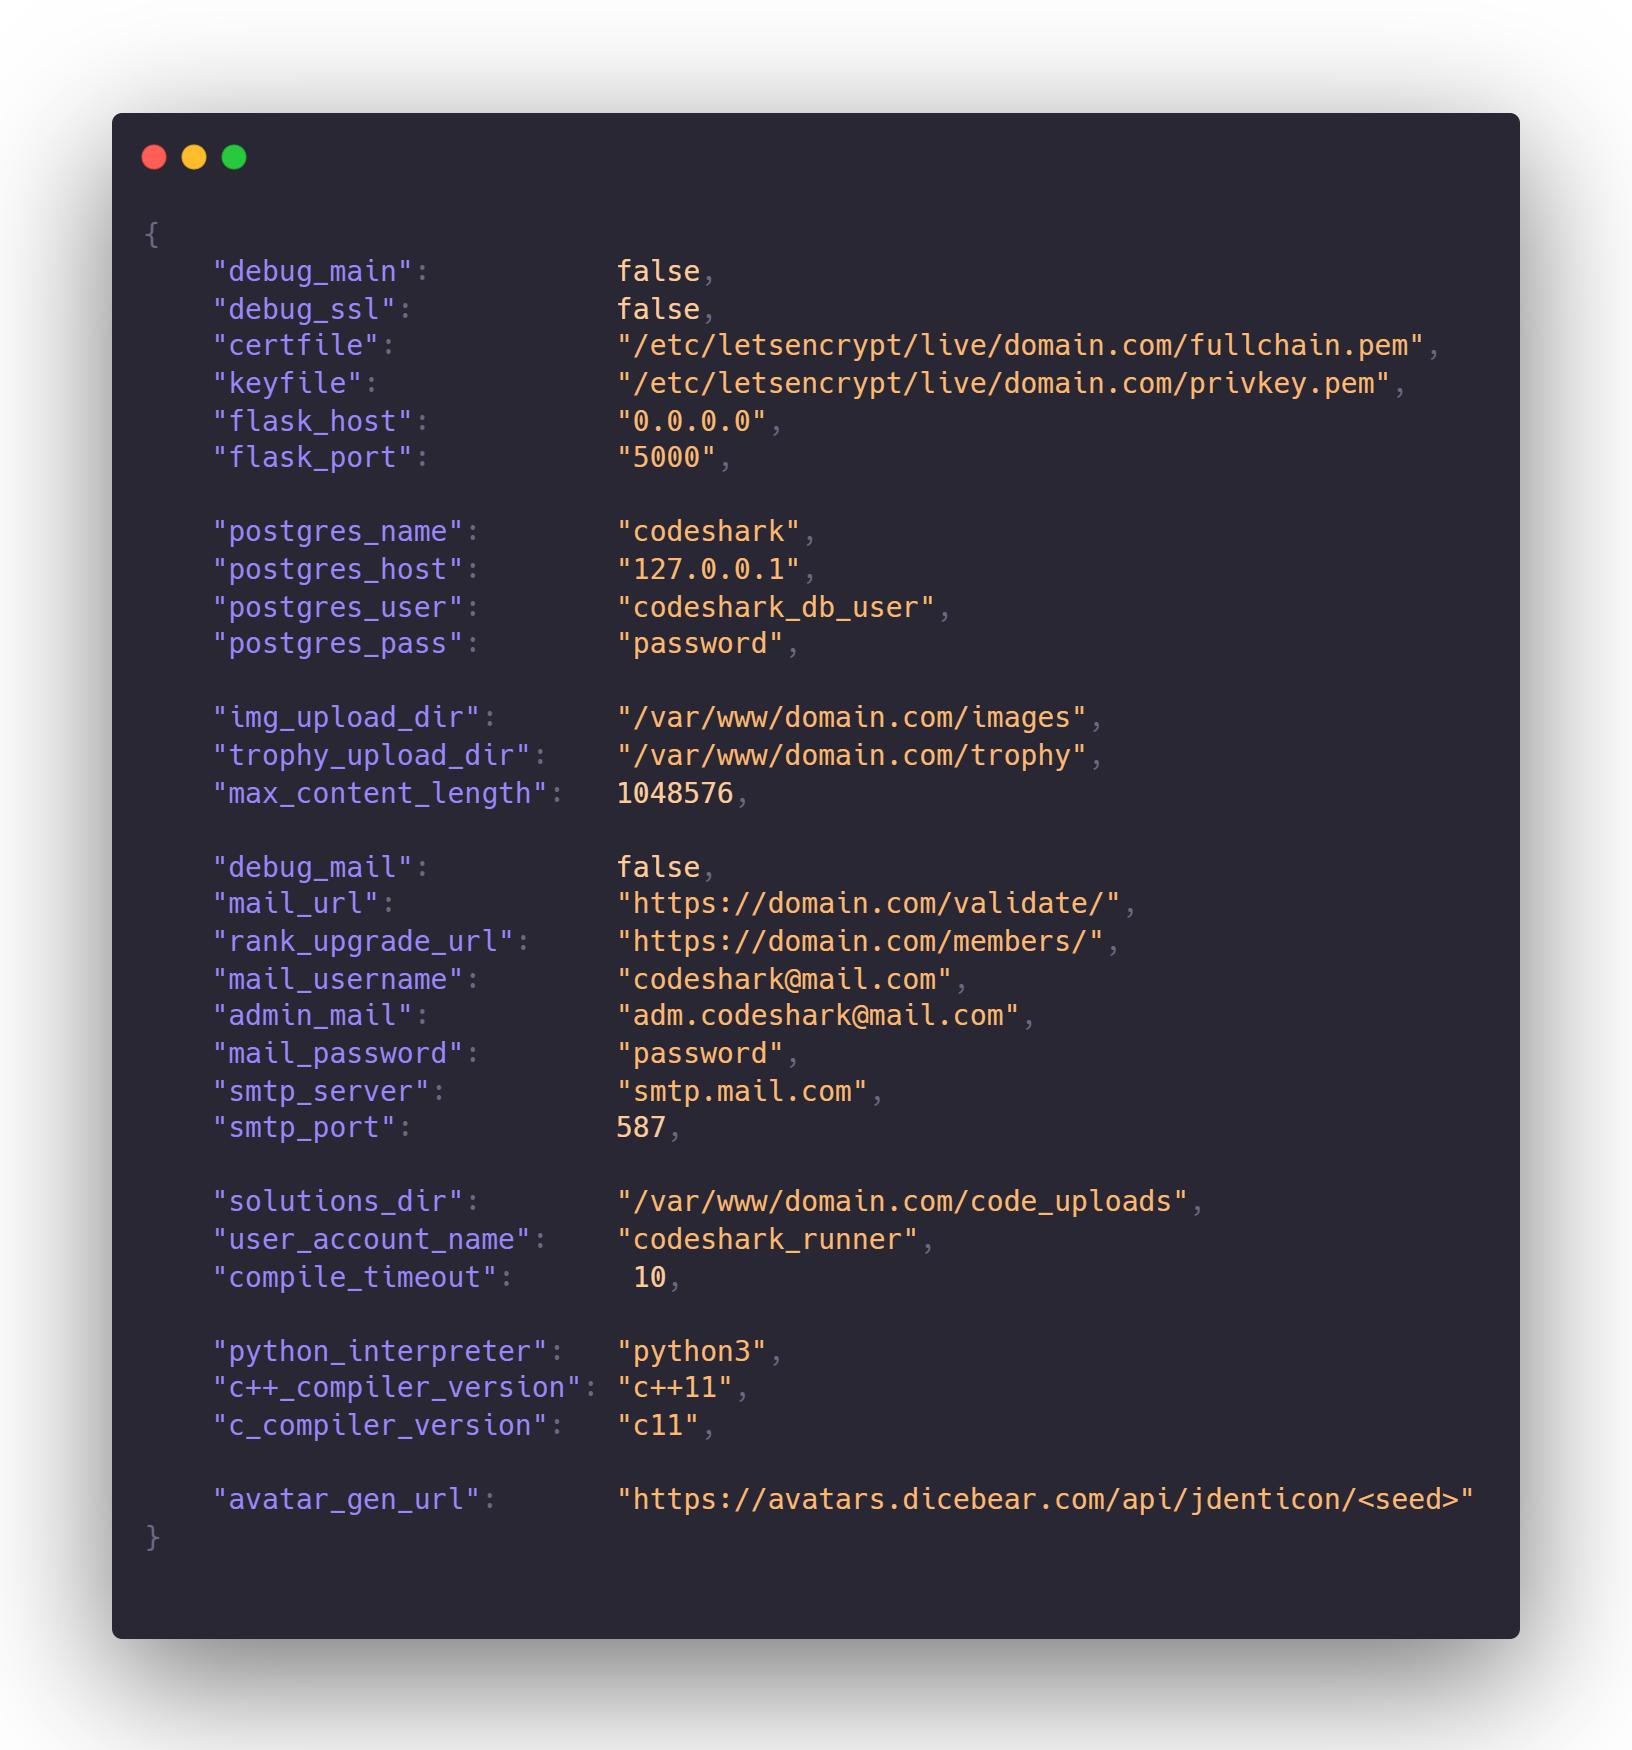
\includegraphics[width=\textwidth]{slike/backendKonfiguracija.png} %veličina u odnosu na širinu linije
				\caption{Primjer konfiguracije backend poslužitelja aplikacije}
				\label{fig:DijagramRazmještaja} %label mora biti drugaciji za svaku sliku
			\end{figure}
			
			
			\textbf{Postavljanje servisa na linux platformi}\\
			
			Održavanje ovakvih aplikacijskih sustava uvelike olakšava mogućnost stvaranja Linux servisa za backend procese. Oni nam omogućavaju jednostavno pokretanje i nadzor nad našim kodom.
			Unutar servisa moguće je specificirati točno na koji način se aplikacija ponaša. Ovdje je bitno obratiti pozornost na korisnika koji izvršava naš kod, njegove dozvole na Linux poslužitelju te putanju do same aplikacije.
			Ovaj dio koda nam omogućava da se čak i u slučaju greške backend sam automatski može ponovno pokrenut. Dodatne pomoćne naredbe bi bile "journalctl -xe -f -u codeshark-testing" pomoću koje u pravom vremenu možemo promatrati izlaz aplikacije, te tako možemo vidjeti trenutno stanje i potencijalne greške tijekom izvođenja.
			
			\begin{figure}[H]
				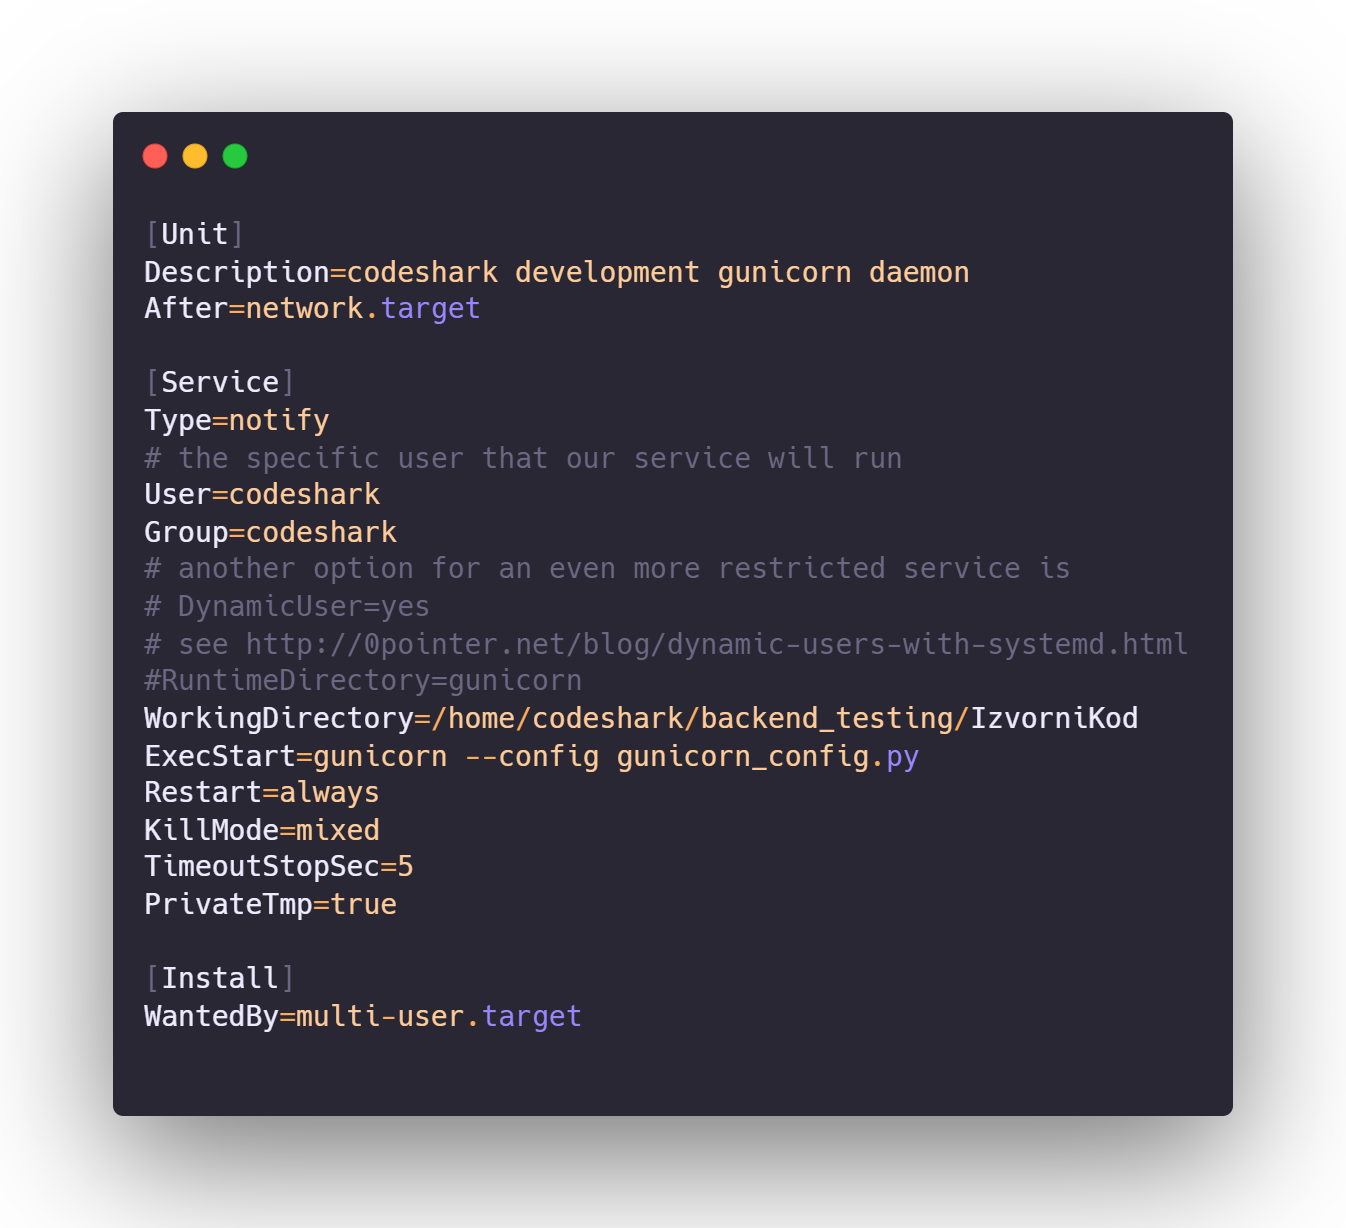
\includegraphics[width=\textwidth]{slike/backendServis.png} %veličina u odnosu na širinu linije
				\caption{Primjer konfiguracije servisa za backend poslužitelja}
				\label{fig:DijagramRazmještaja} %label mora biti drugaciji za svaku sliku
			\end{figure}
			
			Ovaj postupak nije potreban za frontend naše aplikacije pošto je naše web sučelje statički izgrađeno - sav potreban JavaScript kod se izvršava kod klijenta u pregledniku te ne postoji potreba za aktivnim procesom na našem poslužitelju.
			
			\eject
			
			
			\eject 